\documentclass[border=10pt]{standalone}
\usepackage{tikz}
\usetikzlibrary{arrows,positioning,shapes.geometric}
\begin{document}
\
\tikzset{every picture/.style={line width=0.75pt}} %set default line width to 0.75pt        

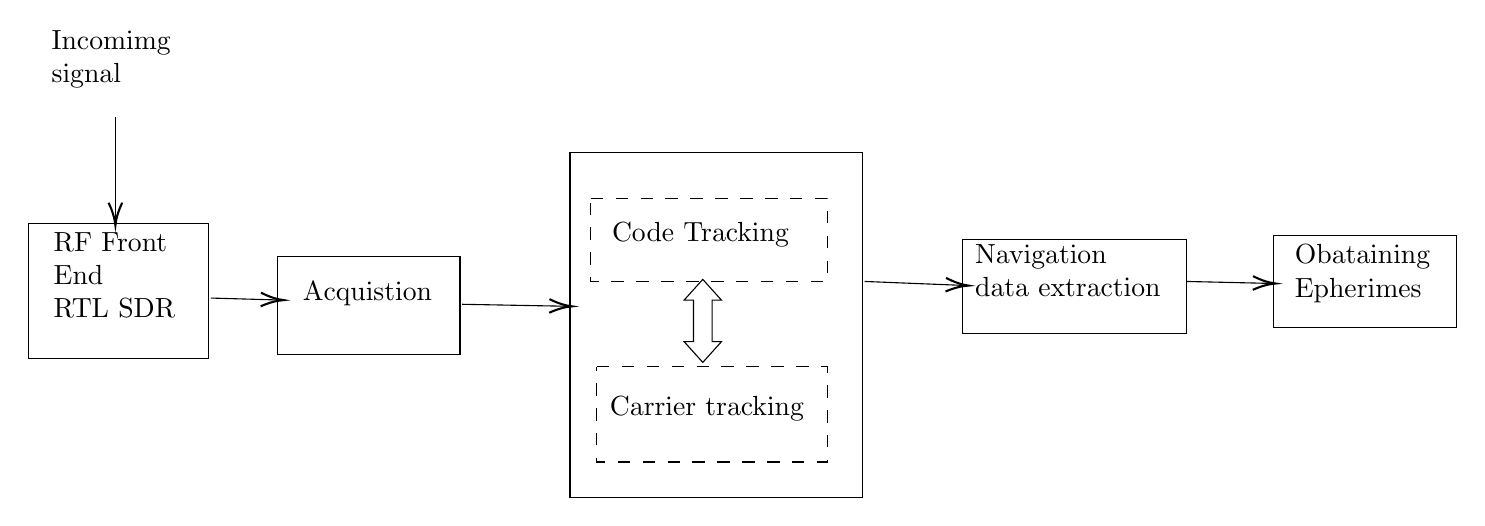
\begin{tikzpicture}[x=0.75pt,y=0.75pt,yscale=-1,xscale=1]
%uncomment if require: \path (0,300); %set diagram left start at 0, and has height of 300

%Shape: Rectangle [id:dp9260211779181345] 
\draw  [dash pattern={on 4.5pt off 4.5pt}] (289,187) -- (400,187) -- (400,233) -- (289,233) -- cycle ;
%Shape: Rectangle [id:dp7949049123793782] 
\draw  [dash pattern={on 4.5pt off 4.5pt}] (286,106) -- (400,106) -- (400,146) -- (286,146) -- cycle ;
%Shape: Rectangle [id:dp0512084112688691] 
\draw   (15,118) -- (102,118) -- (102,183) -- (15,183) -- cycle ;
%Shape: Rectangle [id:dp43686047035032194] 
\draw   (135,134) -- (223,134) -- (223,181) -- (135,181) -- cycle ;
%Shape: Rectangle [id:dp38781321419296166] 
\draw   (465,126) -- (573,126) -- (573,171) -- (465,171) -- cycle ;
%Shape: Rectangle [id:dp5002258739186534] 
\draw   (615,124) -- (703,124) -- (703,168) -- (615,168) -- cycle ;
%Shape: Rectangle [id:dp4513201958133548] 
\draw   (276,84) -- (417,84) -- (417,250) -- (276,250) -- cycle ;
%Straight Lines [id:da8107903345547343] 
\draw    (57,67) -- (57,117) ;
\draw [shift={(57,119)}, rotate = 270] [color={rgb, 255:red, 0; green, 0; blue, 0 }  ][line width=0.75]    (10.93,-3.29) .. controls (6.95,-1.4) and (3.31,-0.3) .. (0,0) .. controls (3.31,0.3) and (6.95,1.4) .. (10.93,3.29)   ;
%Straight Lines [id:da832889164908773] 
\draw    (103,154) -- (136,154.94) ;
\draw [shift={(138,155)}, rotate = 181.64] [color={rgb, 255:red, 0; green, 0; blue, 0 }  ][line width=0.75]    (10.93,-3.29) .. controls (6.95,-1.4) and (3.31,-0.3) .. (0,0) .. controls (3.31,0.3) and (6.95,1.4) .. (10.93,3.29)   ;
%Straight Lines [id:da374925977240681] 
\draw    (224,157) -- (275,157.96) ;
\draw [shift={(277,158)}, rotate = 181.08] [color={rgb, 255:red, 0; green, 0; blue, 0 }  ][line width=0.75]    (10.93,-3.29) .. controls (6.95,-1.4) and (3.31,-0.3) .. (0,0) .. controls (3.31,0.3) and (6.95,1.4) .. (10.93,3.29)   ;
%Up Down Arrow [id:dp32008089080325663] 
\draw   (331,155) -- (340,145) -- (349,155) -- (344.5,155) -- (344.5,175) -- (349,175) -- (340,185) -- (331,175) -- (335.5,175) -- (335.5,155) -- cycle ;
%Straight Lines [id:da5006458459231241] 
\draw    (418,146) -- (440.92,146.92) -- (466,147.92) ;
\draw [shift={(468,148)}, rotate = 182.29] [color={rgb, 255:red, 0; green, 0; blue, 0 }  ][line width=0.75]    (10.93,-3.29) .. controls (6.95,-1.4) and (3.31,-0.3) .. (0,0) .. controls (3.31,0.3) and (6.95,1.4) .. (10.93,3.29)   ;
%Straight Lines [id:da36753033139627644] 
\draw    (573,146) -- (614,146.95) ;
\draw [shift={(616,147)}, rotate = 181.33] [color={rgb, 255:red, 0; green, 0; blue, 0 }  ][line width=0.75]    (10.93,-3.29) .. controls (6.95,-1.4) and (3.31,-0.3) .. (0,0) .. controls (3.31,0.3) and (6.95,1.4) .. (10.93,3.29)   ;

% Text Node
\draw (26,121) node [anchor=north west][inner sep=0.75pt]   [align=left] {RF Front \\End \\RTL SDR};
% Text Node
\draw (146,145) node [anchor=north west][inner sep=0.75pt]   [align=left] {Acquistion};
% Text Node
\draw (295,116) node [anchor=north west][inner sep=0.75pt]   [align=left] {Code Tracking};
% Text Node
\draw (294,200) node [anchor=north west][inner sep=0.75pt]   [align=left] {Carrier tracking};
% Text Node
\draw (470,127) node [anchor=north west][inner sep=0.75pt]   [align=left] {Navigation \\data extraction};
% Text Node
\draw (624,127) node [anchor=north west][inner sep=0.75pt]   [align=left] {Obataining \\Epherimes};
% Text Node
\draw (25,24) node [anchor=north west][inner sep=0.75pt]   [align=left] {Incomimg \\signal};


\end{tikzpicture}

   
\end{document}


